%!TEX program = lualatex
\documentclass[11pt,class=book]{standalone}
%!TEX root = ./main.tex
%!TEX encoding = UTF-8 Unicode

% Pro­gram­ming fa­cil­i­ties
\usepackage{etoolbox}
\usepackage{ifxetex}
\usepackage{ifluatex}

% Encoding
\usepackage[T1]{fontenc}
\ifboolexpr{bool{xetex} or bool{luatex}}{%
	\usepackage{fontspec}
}{%
	\usepackage[utf8]{inputenc}
}

% General purpose
\usepackage{tcolorbox}

% Mathematics
\usepackage{amsmath}
\usepackage{amssymb}
\usepackage{mathrsfs}
\usepackage{amsthm}
\usepackage{dsfont}
\usepackage{braket}
\usepackage{stmaryrd}

% Tables
\usepackage{array}
\usepackage{tabularx}
\usepackage{longtable}
\usepackage{tabu}
\usepackage{booktabs}
\usepackage{multirow}
\usepackage{makecell}
\usepackage{blkarray}

% Figures
\usepackage[mode=tex]{standalone}
\usepackage{import}
\usepackage{float}
\usepackage[justification=centering]{caption}

% PGF-TikZ
\usepackage{pgf}
\usepackage{pgfplots}
\pgfplotsset{compat=1.16}
\usepackage{tikz}
\usepackage{tikzpeople}
\usepackage{pgf-umlsd}
\usepackage{pgfgantt}

%!TEX encoding = UTF-8 Unicode

\usetikzlibrary{shapes}
\usetikzlibrary{arrows.meta}
\usetikzlibrary{calc}

\definecolor{bg_color}{RGB}{250,250,229}

\colorlet{color1}{cyan!50}
\colorlet{color2}{red!30!green!40}
\colorlet{color3}{orange!50}
\colorlet{color4}{violet!60!blue!55}

\definecolor{Cblue}{RGB}{38,75,150}
\definecolor{Cgreen}{RGB}{39,179,118}
\definecolor{Cdarkgreen}{RGB}{0,111,60}
\definecolor{Corange}{RGB}{249,167,62}
\definecolor{Cred}{RGB}{191,33,47}

\newganttlinktype{bartobardown}{
	\ganttsetstartanchor{south east}
	\ganttsetendanchor{north west}
	\draw [/pgfgantt/link] (\xLeft, \yUpper) -- (\xRight, \yLower);
}
\newganttlinktype{bartobarup}{
	\ganttsetstartanchor{north east}
	\ganttsetendanchor{south west}
	\draw [/pgfgantt/link] (\xLeft, \yUpper) -- (\xRight, \yLower);
}
\newganttlinktype{milestonetobardown}{
	\ganttsetstartanchor{south}
	\ganttsetendanchor{north west}
	\draw [/pgfgantt/link] (\xLeft, \yUpper) -- (\xRight, \yLower);
}
\newganttlinktype{bartomilestonedown}{
	\ganttsetstartanchor{south east}
	\ganttsetendanchor{north}
	\draw [/pgfgantt/link] (\xLeft, \yUpper) -- (\xRight, \yLower);
}


\begin{document}
	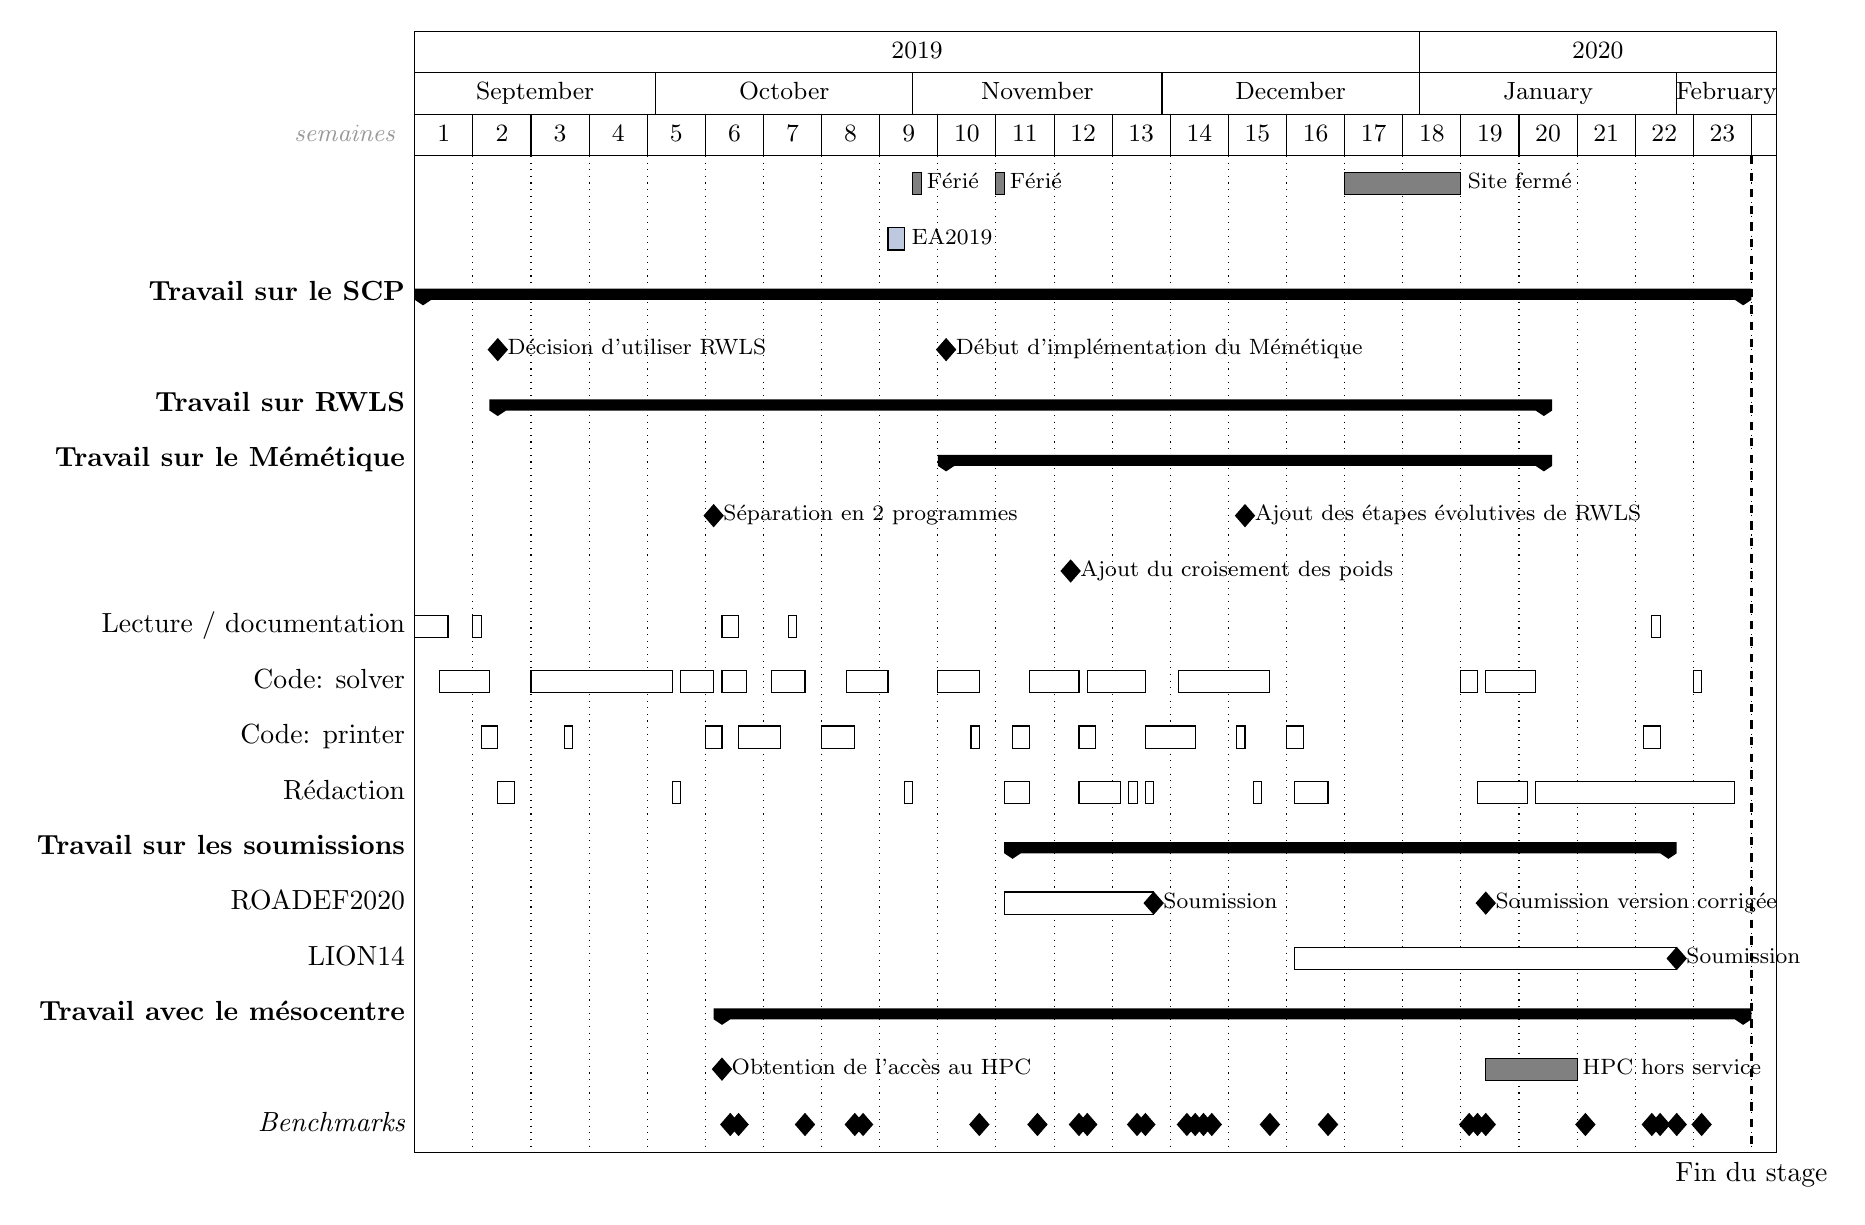
\begin{tikzpicture}[x=1pt,y=1pt]
		\begin{ganttchart}[
				vgrid,
				vgrid={*6{draw=none},*1{dotted}},
				x unit=3,
				y unit chart=20,
				y unit title=15,
				title height=1,
				group left shift=0,
				group right shift=0,
				group peaks width=2,
				link bulge=2.5,
				milestone inline label node/.append style={
					anchor=west,font=\footnotesize
				},
				bar inline label node/.append style={
					font=\footnotesize
				},
				time slot format=isodate,
				milestone/.append style={text width=7},
			]{2019-09-02}{2020-02-12}

			%---------------------------------
			% Time
			\gantttitlecalendar{year,month=name}\\
			\gantttitle[
				title label node/.append style={
					xshift=-25
				}
			]{\color{gray!80}\textit{semaines}}{0}
			\gantttitlelist{1,...,23}{7}
			\gantttitle{}{3}\\

			%---------------------------------
			% Events
			\ganttbar[
				name=closed,
				inline,
				bar/.append style={
					fill=gray
				},
				bar inline label node/.append style={
					anchor=west,
					xshift=0
				}
			]{Férié}{2019-11-01}{2019-11-01}
			\ganttbar[
				name=closed,
				inline,
				bar/.append style={
					fill=gray
				},
				bar inline label node/.append style={
					anchor=west,
					xshift=0
				}
			]{Férié}{2019-11-11}{2019-11-11}
			\ganttbar[
				name=closed,
				inline,
				bar/.append style={
					fill=gray
				},
				bar inline label node/.append style={
					anchor=west,
					xshift=20
				}
			]{Site fermé}{2019-12-23}{2020-01-05}\\
			\ganttbar[
				name=closed,
				inline,
				bar/.append style={
					fill=Cblue!30
				},
				bar inline label node/.append style={
					anchor=west,
					xshift=2
				}
			]{EA2019}{2019-10-29}{2019-10-30}\\

			%---------------------------------
			% Travail sur le SCP
			\ganttgroup{Travail sur le SCP}{2019-09-02}{2020-02-09}
			\\
			%\ganttmilestone[inline]{Début d'implémentation de RWLS}{2019-09-16}
			\ganttmilestone[inline]{Décision d'utiliser RWLS}{2019-09-11}
			\ganttmilestone[inline]{Début d'implémentation du Mémétique}{2019-11-04}
			\\
			\ganttgroup{Travail sur RWLS}{2019-09-11}{2020-01-16}
			\\
			\ganttgroup{Travail sur le Mémétique}{2019-11-04}{2020-01-16}
			\\
			\ganttmilestone[inline]{Séparation en 2 programmes}{2019-10-07}
			\ganttmilestone[inline]{Ajout des étapes évolutives de RWLS}{2019-12-10}\\
			\ganttmilestone[inline]{Ajout du croisement des poids}{2019-11-19}
			\\
			% libcommon = solver + printer
			\ganttbar[name=read]{Lecture / documentation}{2019-09-02}{2019-09-05}
			\ganttbar[inline]{}{2019-09-09}{2019-09-09}
			\ganttbar[inline]{}{2019-10-09}{2019-10-10}
			\ganttbar[inline]{}{2019-10-17}{2019-10-17}
			\ganttbar[inline]{}{2019-01-15}{2019-01-17}
			\ganttbar[inline]{}{2020-01-29}{2020-01-29}
			\\
			\ganttbar{Code: solver}{2019-09-05}{2019-09-10}
			\ganttbar[inline]{}{2019-09-16}{2019-10-02}
			\ganttbar[inline]{}{2019-10-04}{2019-10-07}
			\ganttbar[inline]{}{2019-10-09}{2019-10-11}
			\ganttbar[inline]{}{2019-10-15}{2019-10-18}
			\ganttbar[inline]{}{2019-10-24}{2019-10-28}
			\ganttbar[inline]{}{2019-11-04}{2019-11-08}
			\ganttbar[inline]{}{2019-11-15}{2019-11-20}
			\ganttbar[inline]{}{2019-11-22}{2019-11-28}
			\ganttbar[inline]{}{2019-12-03}{2019-12-13}
			\ganttbar[inline]{}{2020-01-06}{2020-01-07}
			\ganttbar[inline]{}{2020-01-09}{2020-01-14}
			\ganttbar[inline]{}{2020-02-03}{2020-02-03}
			\\
			\ganttbar{Code: printer}{2019-09-10}{2019-09-11}
			\ganttbar[inline]{}{2019-09-20}{2019-09-20}
			\ganttbar[inline]{}{2019-10-07}{2019-10-08}
			\ganttbar[inline]{}{2019-10-11}{2019-10-15}
			\ganttbar[inline]{}{2019-10-21}{2019-10-24}
			\ganttbar[inline]{}{2019-11-08}{2019-11-08}
			\ganttbar[inline]{}{2019-11-13}{2019-11-14}
			\ganttbar[inline]{}{2019-11-21}{2019-11-22}
			\ganttbar[inline]{}{2019-11-29}{2019-12-04}
			\ganttbar[inline]{}{2019-12-10}{2019-12-10}
			\ganttbar[inline]{}{2019-12-16}{2019-12-17}
			\ganttbar[inline]{}{2020-01-28}{2020-01-29}
			\\
			\ganttbar{Rédaction}{2019-09-12}{2019-09-13}
			\ganttbar[inline]{}{2019-10-03}{2019-10-03}
			\ganttbar[inline]{}{2019-10-31}{2019-10-31}
			\ganttbar[inline]{}{2019-11-12}{2019-11-14}
			\ganttbar[inline]{}{2019-11-21}{2019-11-25}
			\ganttbar[inline]{}{2019-11-27}{2019-11-27}
			\ganttbar[inline]{}{2019-11-29}{2019-11-29}
			\ganttbar[inline]{}{2019-12-12}{2019-12-12}
			\ganttbar[inline]{}{2019-12-17}{2019-12-20}
			\ganttbar[inline]{}{2020-01-08}{2020-01-13}
			\ganttbar[inline]{}{2020-01-15}{2020-02-07}
			\\

			%---------------------------------
			% Travail sur les soumissions
			%\ganttnewline[dashed]
			\ganttgroup{Travail sur les soumissions}{2019-11-12}{2020-01-31}
			\\
			%\ganttmilestone[inline,name=droadef]{Désicion de soumettre}{2019-11-12}\\
			\ganttbar[name=roadef]{ROADEF2020}{2019-11-12}{2019-11-29}
			\ganttmilestone[inline]{Soumission}{2019-11-29}
			\ganttmilestone[inline]{Soumission version corrigée}{2020-01-08}
			\\
			%\ganttmilestone[inline,name=dlion]{Désicion de soumettre}{2019-12-17}\\
			\ganttbar[name=lion]{LION14}{2019-12-17}{2020-01-31}
			\ganttmilestone[inline]{Soumission}{2020-01-31}
			\\
			%\ganttlink[link type=milestonetobardown]{droadef}{roadef}
			%\ganttlink[link type=milestonetobardown]{dlion}{lion}

			%---------------------------------
			% Travail avec le mésocentre
			%\ganttnewline[dashed]
			\ganttgroup{Travail avec le mésocentre}{2019-10-08}{2020-02-09}\\
			\ganttmilestone[inline]{Obtention de l'accès au HPC}{2019-10-08}
			\ganttbar[
				name=closed,
				inline,
				bar/.append style={
					fill=gray
				},
				bar inline label node/.append style={
					anchor=west,
					xshift=15
				}
			]{HPC hors service}{2020-01-09}{2020-01-19}\\
			\ganttmilestone{Benchmarks}{2019-10-09}
			\ganttmilestone[inline]{}{2019-10-10}
			\ganttmilestone[inline]{}{2019-10-18}
			\ganttmilestone[inline]{}{2019-10-24}
			\ganttmilestone[inline]{}{2019-10-25}
			\ganttmilestone[inline]{}{2019-11-08}
			\ganttmilestone[inline]{}{2019-11-15}
			\ganttmilestone[inline]{}{2019-11-20}
			\ganttmilestone[inline]{}{2019-11-21}
			\ganttmilestone[inline]{}{2019-11-28}
			\ganttmilestone[inline]{}{2019-11-27}
			\ganttmilestone[inline]{}{2019-12-03}
			\ganttmilestone[inline]{}{2019-12-04}
			\ganttmilestone[inline]{}{2019-12-05}
			\ganttmilestone[inline]{}{2019-12-06}
			\ganttmilestone[inline]{}{2019-12-13}
			\ganttmilestone[inline]{}{2019-12-20}
			\ganttmilestone[inline]{}{2020-01-06}
			\ganttmilestone[inline]{}{2020-01-07}
			\ganttmilestone[inline]{}{2020-01-08}
			\ganttmilestone[inline]{}{2020-01-20}
			\ganttmilestone[inline]{}{2020-01-28}
			\ganttmilestone[inline]{}{2020-01-29}
			\ganttmilestone[inline]{}{2020-01-31}
			\ganttmilestone[inline]{}{2020-02-03}

			%---------------------------------
			% events
			% \\\ganttnewline[dashed]\\
			% \ganttmilestone[inline]{Présentation du travail de 8INF870}{2019-09-04}\\
			% \ganttmilestone[inline]{Début de l'implémentation du solver}{2019-09-05}\\
			% \ganttmilestone[inline]{Début de l'implémentation du greedy}{2019-09-06}\\
			% \ganttmilestone[inline]{Début de l'implémentation du printer}{2019-09-10}\\
			% \ganttmilestone[inline]{Décision d'utiliser RWLS}{2019-09-11}\\
			% \ganttmilestone[inline]{Envoi du projet de stage}{2019-09-15}\\
			% \ganttmilestone[inline]{Début d'implémentation de RWLS}{2019-09-16}\\
			% \ganttmilestone[inline]{Début d'implémentation du système de lancement}{2019-09-20}\\
			% \ganttmilestone[inline]{Introduction des rapports d'exécussion}{2019-09-25}\\
			% \ganttmilestone[inline]{Début d'implémentation de la réduction des instances}{2019-09-27}\\
			% \ganttmilestone[inline]{Demande d'accès au mésocentre}{2019-10-01}\\
			% \ganttmilestone[inline]{Introduction de la PGO}{2019-10-04}\\
			% \ganttmilestone[inline]{Début de l'implémentation du printer}{2019-10-07}\\
			% \ganttmilestone[inline]{Accès au mésocentre}{2019-10-08}\\
			% \ganttmilestone[inline]{Premiers résultats de RWLS}{2019-10-14}\\
			% \ganttmilestone[inline]{Premieres statistiques sur RWLS}{2019-10-23}\\
			% \ganttmilestone[inline]{Création des dépots d'instances et de résultats}{2019-10-31}\\
			% \ganttmilestone[inline]{Début d'implémentation du Mémétique}{2019-11-04}\\
			% \ganttmilestone[inline]{Désicion de soumettre pour ROADEF2020}{2019-11-12}\\
			% \ganttmilestone[inline]{Ajout du croisement des poids des points}{2019-11-19}\\
			% \ganttmilestone[inline]{Début d'implémentation du système de cache de réduction}{2019-11-25}\\
			% \ganttmilestone[inline]{Soumission ROADEF2020}{2019-11-29}\\
			% \ganttmilestone[inline]{Début d'implémentation des graphiques de poids}{2019-11-29}\\
			% \ganttmilestone[inline]{Début d'implémentation des étapes évolutives de RWLS}{2019-12-10}\\
			% \ganttmilestone[inline]{Début d'implémentation des graphes de répartition des solutions}{2019-12-17}\\
			% \ganttmilestone[inline]{Désicion de soumettre pour LION14}{2019-12-17}\\
			% \ganttmilestone[inline]{Soumission finale ROADEF2020}{2020-01-08}\\
			% \ganttmilestone[inline]{Début d'implémentation du support des instances GVCP}{2020-01-13}\\
			% \ganttmilestone[inline]{Soumission LION14}{2020-01-31}\\

			% \ganttvrule[
			% 	vrule/.append style={thin,solid},
			% ]{}{2019-10-31}
			% \ganttvrule[
			% 	vrule/.append style={thin,solid},
			% ]{}{2019-11-01}

			% \ganttvrule[
			% 	vrule/.append style={thin,solid},
			% ]{}{2019-11-10}
			% \ganttvrule[
			% 	vrule/.append style={thin,solid},
			% ]{}{2019-11-11}

			% \ganttvrule[
			% 	vrule/.append style={thin,solid},
			% ]{}{2019-12-22}
			% \ganttvrule[
			% 	vrule/.append style={thin,solid},
			% ]{}{2020-01-05}

			\ganttvrule[
%				vrule/.append style={red, thin},
%				vrule offset=.2,
%				vrule label node/.append style={anchor=north west}
			]{Fin du stage}{2020-02-09}
		\end{ganttchart}
	\end{tikzpicture}
\end{document}
